\chapter{Managing Supply Under Demand-Side Parameter Uncertainty}

First, we solve a simpler problem that involves parameter uncertainty only on the demand side. We would later extend these findings to supply side parameter uncertainty. This problem is more complicated than it sounds. In every day life, the arrival rates are uncertain. However, most of the traditional literature assumes that all model primitives are known with certainty, and “noise” is restricted to stochastic variability. 

\section{Reviewing Existing Models}
There are mainly 2 key factors considered to make the choice of capacity level: 
\begin{enumerate}
  \item \textbf{Efficiency:} This concerns itself with basic operating costs, e.g, factors like cost of hiring play an important role.
  \item \textbf{Quality:} This concerns itself with quality of customer service, e.g., factors like abandonment costs play an important role. 
\end{enumerate}
 
 Capacity planning is a trade-off between these 2 factors. The best quality of service would require a high amount of spare capacity which could be wasteful and the best efficiency would require preventing occurrence of idle servers this can greatly degrade the quality of service. \\ \\
If the arrivals follow a Poisson process with rate $\lambda$ and services are exponentially distributed with rate $\mu$. \\
Some common regimes that are in use give the capacity C as:
\begin{enumerate}
  \item \textbf{Efficiency-Driven (ED) Regime:}
  \[ C = \frac{\lambda}{\mu} - \gamma\frac{\lambda}{\mu} \ \ where \ \ 0 < \gamma < 1\]
  This model is likely to be under-staffed.
  \item \textbf{Quality-Driven (QD) Regime:} 
  \[ C = \frac{\lambda}{\mu} + \delta\frac{\lambda}{\mu} \ \ where \ \ \delta >0\]
  This model is likely to be over-staffed.
  \item \textbf{Quality- and Efficiency-Driven (QED) Regime:} 
  \[ C = \frac{\lambda}{\mu} + \beta\sqrt{\frac{\lambda}{\mu}} \ \ where \ \ -\infty<\beta<\infty\]
  This regime is also known as the Halfin-Whitt regime \cite{qedRegime}.
\end{enumerate}
In all the cases above, the term $\frac{\lambda}{\mu}$ is a base capacity used to meet mean demands. The second term is the variability hedge. The QED regime is popular because it takes into account both the quality and efficiency factors. It takes the form dictated by the The Square Root Staffing Law that was covered in the Key Concepts chapter. \\

However, the QED regime is not very good for practical implementation. The square-root-law expects a fairly accurate estimate of the service and arrival rates. However, in a practical setting, such parameters are estimated and predicted on the basis of historical data, and hence can be quite “noisy.” That means there is expected to be ambiguity in the parameters, such as, arrival rate itself. Hence, we try to find a better solution to the problem.

\section{Proposing an Approximate Solution based on the Newsvendor Problem}
\subsection{Formulating the Problem}
\begin{itemize}
\itemsep0em
  \item \textbf{Servers:} $b$ identical servers
  \item \textbf{Customer Arrivals:} Doubly stochastic Poisson process, that is, the arrival rate $\Lambda$ is also a random variable. It has distribution F and mean $\lambda$. The arrival process is a homogeneous Poisson process with this rate.
  \item \textbf{Service Requirements:} i.i.d. exponential random variables. They are independent of the arrival process and rate and have mean $\frac{1}{\mu}$
  \item \textbf{Queue Discipline:} FCFS (First come first served) is used. 
  \item \textbf{Waiting Policy:} Servers do not remain idle unless queue is empty. There is an infinite capacity buffer. The per-customer per-unit-time cost of a customer waiting in queue is called the holding cost and it is h per customer per unit time.  
  \item \textbf{Abandonment Policy:} Customers have the impatience random variable $\tau$, exponentially distributed with mean $\frac{1}{\gamma}$. A customer may abandon the system after getting impatient from waiting. The customer will abandon the system when her total waiting time in queue reaches $\tau$ time units. There is a cost incurred at a rate p per customer, this is called the abandonment cost. 
  \item \textbf{Staffing Cost:} c per unit time per server.
  \item \textbf{Queuing Model:} $M/M/b +M$ with a random arrival rate.
  \item $N$ is the random variable that represents the number of customers in the system in steady state. 
  \item Length of the planning horizon is normalized to 1.
  \item Integrality constraints are ignored and $b$ is assumed to be real-valued.
\end{itemize}

Putting things together, \\
Expected Steady State Queue length = $\mathbb{E}[N - b]^+$. \\
Cost related to Quality, or the total expected customer cost in steady state = $(h + p\gamma)\mathbb{E}[N - b]^+$. \\
Cost related to Efficiency, or the total staffing cost = $cb$.\\ \\
\textbf{The Optimization Problem:}\\ 
\[Minimize \ \ \Pi(b)=(h + p\gamma)\mathbb{E}[N - b]^+ + cb\]     
\[subject \ \ to \ \ b \geq 0\]    
\\
Let $b^*$ denote the minimizer and $\Pi^* := \Pi(b^*)$ the corresponding minimum cost.
\subsection{Proposing an Approximate Solution}
The optimization problem looks simple. However, it is not possible to get an exact solution to it. This is because the distribution of $N$ itself depends on $b$. \\
\textbf{Approach:} We ignore the stochastic variability in customer arrivals and service requirements. We only focus our attention on the uncertainty in the arrival rate. This relaxation makes things easy because now customer arrivals form a fluid queue with the fluid flowing at the rate $\Lambda$ per unit time. The processing
capacity is is equal to $\mu$b and is fixed. \\
\[Rate \ \ of \ \ Abandonment \approx \mathbb{E}[\Lambda - \mu b]^+\] \\
Also, 
\[Rate \ \ of \ \ Abandonment = \gamma\mathbb{E}[N - b]^+\]
So,
\[\mathbb{E}[N - b]^+ \approx \frac{1}{\gamma} \mathbb{E}[\Lambda - \mu b]^+ \ \ \ \ \ \cite{bassamboo}  \] 
This helps us get rid of N which was causing some problems. Now, \\ \\
\textbf{The Optimization Problem:}\\ 
\[Minimize \ \ \bar{\Pi}(b)=(p + \frac{h}{\gamma})\mathbb{E}[\Lambda - \mu b]^+ + cb\]     
\[subject \ \ to \ \ b \geq 0\]     
Here, $\bar{\Pi}(.)$ is the new objective function that is being proposed. \\
This is an instance of the newsvendor problem that was visited in the Key Concepts chapter where $C=\frac{c}{\mu} \ \ and \ \ P=p + \frac{h}{\gamma} \ \ and \ \ S=0$. Also, the Number of Units available is analogous to the Processing Capacity available. So, $Q=\mu b$. If F is the cumulative distribution function of $\Lambda$, then, $\bar{F}$ = 1 - F.
So, \\
\[\bar{Q}=F^{-1}(\frac{P-C}{P-S})\]
\[\bar{Q}=F^{-1}(\frac{P-C}{P-0})=F^{-1}(\frac{P-C}{P})\]
\[\bar{Q}=\bar{F}^{-1}(\frac{C}{P})\]
\[\mu \bar{b}=\bar{F}^{-1}(\frac{\frac{c}{\mu}}{p + \frac{h}{\gamma}})\]
\[\bar{b}=\frac{1}{\mu}\bar{F}^{-1}(\frac{\frac{c}{\mu}}{p + \frac{h}{\gamma}})\]
\begin{remark}
Note that if the cost of capacity (per unit) is higher than the penalty charge (per unit), the optimal solution would not install any capacity. Our proposed solution would not install any capacity either.
More formally,
If,
\[\frac{c}{\mu}>p + \frac{h}{\gamma}\]
Then,
\[b^*=\bar{b}=0\]
\end{remark}
\section{Analysing the Performance of the Proposed Solution}
We will be using some numerical data to analyse the performance of the proposed solution relative to the optimal solution. For all the cases we consider $c=1/3$, $p=1$, $h=1$, $\mu=1$ and $\gamma=1/3$. These values ensure that the condition of Remark 2.2.1 does not arise. In all the cases, the optimal solution has been picked from the internet and the proposed solution is computed using the formula derived in section 2.2.2. All values have been rounded to 1 decimal place. \\
After forming our intuitions based on the numerical data we mention some related mathematical results that justify our observations. These relations are derived in Bassamboo and Randhawa (2010) \cite{bassamboo} and are stated here without proof. \\
Before moving further, a few terms need to be defined that will be used in this section. 
\begin{definition}\label{}
The safety capacity ($\beta$) is defined as the difference between the optimal solution $b^*$ and the proposed solution $\bar{b}$.
\end{definition}
\begin{definition}\label{}
The accuracy gap ($\Delta(b)$) is defined as the difference between the value of the actual objective function at b, $\Pi(b)$, and the value of the proposed newsvendor objective function at b, $\bar{\Pi}(b)$.
\end{definition}
\begin{definition}\label{}
The optimality gap is defined as the difference between the value of $\Pi(\bar{b})$ and the value of $\Pi(b^*)$.
\end{definition}
\subsection{Deterministic Arrival Rates}
We first consider the simple case where there is no uncertainty in the arrival rate, that is, the case where arrival rate takes constant values. \\ \\
\textbf{Computing the Proposed Solution}\\
\[\bar{b}=\frac{1}{\mu}\bar{F}^{-1}(\frac{\frac{c}{\mu}}{p + \frac{h}{\gamma}})\]
\[\bar{b}=\frac{1}{1}\bar{F}^{-1}(\frac{\frac{1/3}{1}}{1 + \frac{1}{1/3}})\]
\[\bar{b}=\bar{F}^{-1}(\frac{1}{12})\]
\[\bar{b}=F^{-1}(\frac{11}{12})\]
Now, for the deterministic case,
\[F^{-1}(p) = \lambda \ \ where \ \ 0<p<1\]
So,
\[\bar{b}= \lambda \]
\textbf{Comparing the Proposed Solution with the Optimal Solution using Numerical Data}\\
Table 2.1 and Figure 2.1 show the performance of the proposed solution on deterministic arrival rates. \\
We see that the optimality gap increases as the value of the arrival rate increases. We see that the gap between $b$ and $b^*$ also increases with increasing arrival rate.

\begin{remark}
When the arrival rate increases by 4 times in the last 2 rows of Table 2.1, we see that the optimality gap approximately doubles. The value of the safety capacity is positive in all cases and it doubles in the aforementioned case. Looking carefully we see that $\beta$ grows proportionally to $\sqrt{\lambda}$. This is very much in line with the square root staffing law, as one would expect in case of deterministic arrivals. 
\end{remark}
\begin{center}
\begin{table}[hbt!]
            \begin{tabular}{|c||c|c|c|c|c|c|}
            \hline
            Arrival Rate &  \multicolumn{2}{|c|}{Optimal Solution} & \multicolumn{2}{|c|}{Proposed Solution}& \multicolumn{2}{|c|}{Comparison} \\
            \hline
                $\lambda$& $b^*$ & $\Pi(b^*)$ & $\bar{b}$& $\Pi(\bar{b})$& $|b^*-\bar{b}|$& Optimality Gap\\ 
                    \hline \hline
                    37.5 & 42 & 15.9 & 37 & 17.7 & 5& 1.7\\
                    75 & 83 & 29.6 & 75 & 31.6 & 8& 2.0\\
                    300 & 316 & 109 & 300 & 112.4 & 16& 3.4\\
            \hline
            \end{tabular} 
            \caption{Performance of the Proposed Solution on Deterministic Arrival Rates}            
\end{table}

\begin{figure}[hbt!]
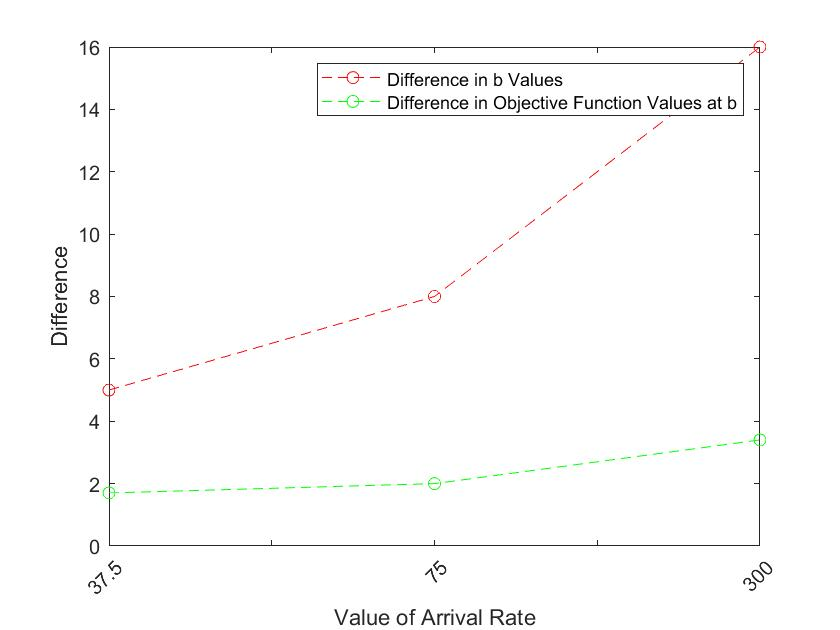
\includegraphics[height=10cm]{correctedDet.jpg}
\caption{Performance of the Proposed Solution on Deterministic Arrival Rates}
\subcaption{This image shows the deviation of the proposed solution from the optimal one in the case of different arrival rate values. }
\subcaption{The red line shows the values of $|b^*-\bar{b}|$ and the green line shows the value of $\Pi(\bar{b})-\Pi(b^*)$.}
\end{figure}
\end{center}
\textbf{Related Mathematical Results}\\
\[b^* \approx \bar{b} + C_0\sqrt{\frac{\lambda}{\mu}} \ \ \ \ and \ \ \ \ \Pi(b^*) \approx \Pi(\bar{b}) -  C_1\sqrt{\frac{\lambda}{\mu}}  \ \ \cite{bassamboo}\]

\subsection{Uncertain Arrival Rates}
We assume that the arrival rates follow a uniform distribution, U[a,b]. \\ \\
\textbf{Computing the Proposed Solution} \\
\[\bar{b}=\frac{1}{\mu}\bar{F}^{-1}(\frac{\frac{c}{\mu}}{p + \frac{h}{\gamma}})\]
\[\bar{b}=\frac{1}{1}\bar{F}^{-1}(\frac{\frac{1/3}{1}}{1 + \frac{1}{1/3}})\]
\[\bar{b}=\bar{F}^{-1}(\frac{1}{12})\]
\[\bar{b}=F^{-1}(\frac{11}{12})\]
Now, for U[a,b],
\[F^{-1}(p) = a + p(b-a) \ \ where \ \ 0<p<1\]
So,
\[\bar{b}=a+\frac{11}{12}(b-a)=\frac{11}{12}b-\frac{1}{12}a\] \\
\textbf{Comparing the Proposed Solution with the Optimal Solution using Numerical Data} \\
Table 2.2 and Figure 2.3 show the performance of the proposed solution on uncertain arrival rates. \\
We observe that the performance is quite bad when the mean arrival rate is small. It improves as we move towards larger mean arrival rates. The drop in the value of optimality gap is, infact, quite drastic in the beginning. We see good performance after U[10,20]. The poor performance in case of smaller mean arrival rates can be ignored in a practical scenario because mostly large traffic is seen.
\begin{remark}
Observe that arrivals rate values in Table 2.1 are nothing but the mean of the distributions in last 3 rows of Table 2.2. The difference in the value of optimality gap in the two tables, however, is quite high. This shows that the proposed solution works better when the arrival rate has uncertainty.
\end{remark}
\begin{center}
\begin{table}[hbt!]
            \begin{tabular}{|c||c|c|c|c|c|c|}
            \hline
            Arrival Rate &  \multicolumn{2}{|c|}{Optimal Solution} & \multicolumn{2}{|c|}{Proposed Solution}& \multicolumn{2}{|c|}{Comparison} \\
            \hline
                Distribution& $b^*$ & $\Pi(b^*)$ & $\bar{b}$& $\Pi(\bar{b})$& $|b^*-\bar{b}|$& Optimality Gap\\ 
                    \hline \hline
                    U[1,2] & 3 & 1.4 & 1 & 5.3 & 2& 3.8\\ 
                    U[2,4] & 5 & 2.2 & 3 & 3.3 & 2& 1.1\\
                    U[5,10] & 11 & 4.3 & 8 & 5.0 & 3& 0.7\\
                    U[10,20] & 20 & 7.7 & 17 & 8.0 & 3& 0.3\\
                    U[15,30] & 29 & 11.0 & 26 & 11.1 & 3& 0.2\\
                    U[20,40] & 37 & 14.2 & 35 & 14.3 & 2& 0.1\\
                    U[25,50] & 46 & 17.3 & 43 & 17.5 & 3& 0.2\\
                    U[50,100] & 89 & 33.1 & 87 & 33.2 & 2& 0.1\\
                    U[200,400] & 351 & 127.1 & 350 & 127.1 & 1& 0.0\\
            \hline
            \end{tabular} 
            \caption{Performance of the Proposed Solution on Uncertain Arrival Rates}            
\end{table}

\begin{figure}[hbt!]
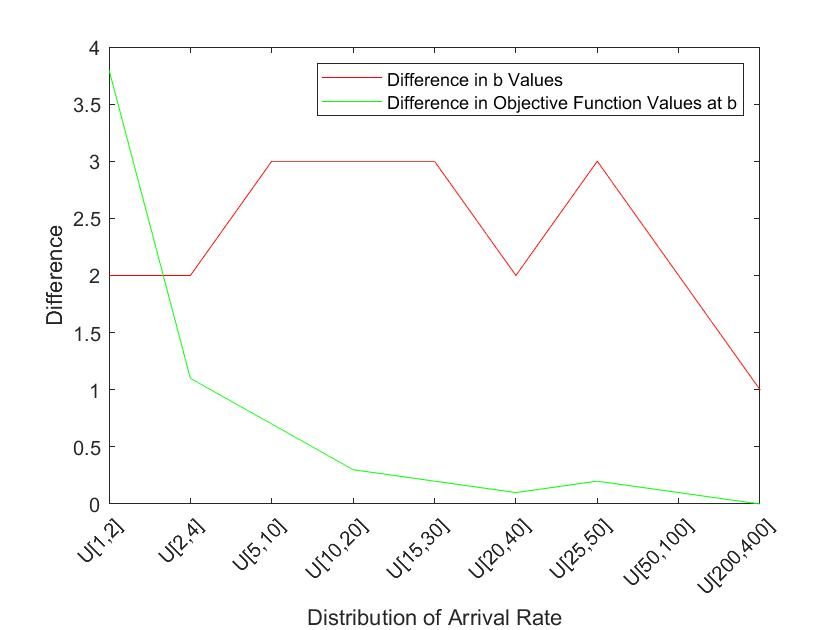
\includegraphics[height=10cm]{correctedUni.jpg}
\caption{Performance of the Proposed Solution on Uncertain Arrival Rates}
\subcaption{This image shows the deviation of the proposed solution from the optimal one in the case of various arrival rate distributions. }
\subcaption{The red line shows the values of $|b^*-\bar{b}|$ and the green line shows the value of $\Pi(\bar{b})-\Pi(b^*)$.}
\end{figure}

\end{center}
\textbf{Related Mathematical Results}\\
\[\Delta(b) = \Pi(b) - \bar{\Pi}(b) \approx K\mathbb{E}\left[\sqrt{\frac{\Lambda}{\mu}}exp(-\frac{(\frac{\Lambda}{\mu}-b)^2}{2\frac{\Lambda}{\mu}})\right] \ \ \cite{bassamboo}\]

\begin{remark}
The exponential term dominates in RHS. This term is clearly small when there is some amount of uncertainty in the arrival rates. This means that minimising $\Pi(b)$ essentially means minimising $\bar{\Pi}(b)$. That is why, in case of uncertainty, the newsvendor solution works very well.   
\end{remark}
\section{Some Important Results}
This section mentions some important results derived in \cite{bassamboo}. These are stated here without proof. In this section, the terms have been appended with an additional subscript $\lambda$ where $\lambda=\mathbb{E}(\Lambda)$ is assumed to be large, as is the case in most practical scenarios. We assume that $\sigma_{\lambda} < \infty$. Some new terms must be defined before moving forward.
\begin{definition}\label{}
The coefficient of variation of the arrival rate ($CV_{\lambda}$) is defined as the ratio of $\sigma_{\lambda}$ and $\lambda$.
\end{definition}

\begin{definition}\label{}
The offered load ($\varepsilon_{\lambda}$) is defined as the ratio of $\lambda$ and $\mu$.
\end{definition}

\begin{theorem} (Performance of the solution in different regimes) \\
(a) (Uncertainty-dominated regime.) If $CV_{\lambda} \gg \frac{1}{\sqrt{\varepsilon_{\lambda}}}$, then, 
\[\Pi_{\lambda}(\bar{b_{\lambda}}) = \Pi_{\lambda}(b_{\lambda}^*) + \mathcal{O}\left(\frac{1}{CV_{\lambda}}\right)\]
(b) (Variability-dominated regime.) If $CV_{\lambda} \ll \frac{1}{\sqrt{\varepsilon_{\lambda}}}$, then, 
\[\Pi_{\lambda}(\bar{b_{\lambda}}) = \Pi_{\lambda}(b_{\lambda}^*) + \mathcal{O}(\sqrt{\varepsilon_{\lambda}})\]
(c) If the variability and uncertainty are balanced, then, 
\[\Pi_{\lambda}(\bar{b_{\lambda}}) = \Pi_{\lambda}(b_{\lambda}^*) + \mathcal{O}(\sqrt{\varepsilon_{\lambda}})\]
(d) (Deterministic regime). If $CV_{\lambda}=0$, then, 
\[\Pi_{\lambda}(\bar{b_{\lambda}}) = \Pi_{\lambda}(b_{\lambda}^*) + \mathcal{O}(\sqrt{\varepsilon_{\lambda}})\]
\end{theorem}

\begin{theorem} (A special case of $\mathcal{O}(1)$ optimality) \\
If $CV_{\lambda}$ is bounded away from zero, then, 
\[\Pi_{\lambda}(\bar{b_{\lambda}}) = \Pi_{\lambda}(b_{\lambda}^*) + \mathcal{O}(1)\]
\end{theorem}